\chapter{卖出看涨期权比率}
\section{卖出看涨期权比率}
简单地说,卖出看涨期权比率(ratio call writing)是这样一种策略,投资者持有一定数量的标的股票,同时他卖出了更多股数的看涨期权。因此,卖出的看涨期权所对应的股数与已持有的股数之间就有了一个比率。最常见的比率是 2:1,在这种比率上,投资者持有 100 股标的股票,同时卖出 2 手看涨期权。请注意,这类头寸涉及卖出一定数量的裸期权以及一定数量的备兑期权。由此而产生的头寸,既有卖出备兑看涨期权时的下行风险,又有裸卖出时的无限上行风险。如果标的股票价格在期权存续期内保持相对无变化,卖出看涨期权比率的盈利会比只卖出备兑看涨期权和只卖出裸看涨期权都要大得多。不过与卖出备兑看涨期权和裸看涨期权不一样,卖出看涨期权比率在两个方向上都面临风险。

一般而言,某个投资者在建立卖出看涨期权比率头寸的时候,他应当对标的股票的前景保持中立。这就是说,他卖出的是行权价最接近当前股票价格的看涨期权。
\begin{figure}
    \centering
    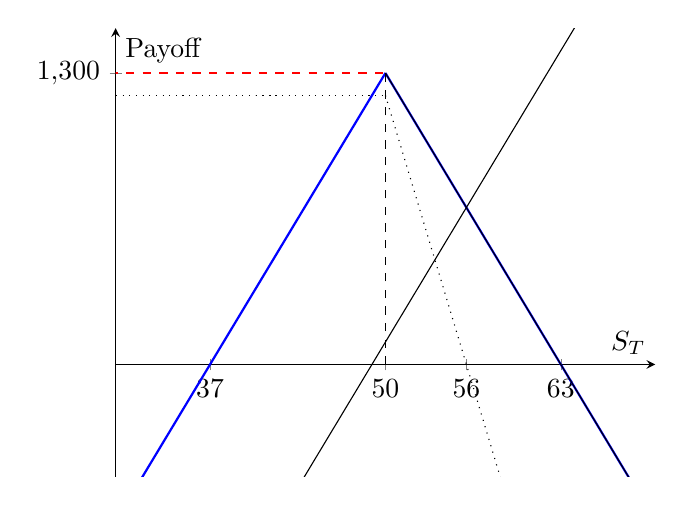
\begin{tikzpicture}
        \begin{axis}[
                axis lines=middle,
                xlabel={$S_T$},
                ylabel={Payoff},
                xmin=30, xmax=70,   % 调整x轴的范围
                ymin=-500, ymax=1500, % 调整y轴的范围
                xtick={37,50,56,63},
                ytick={1300},
                domain=0:100, % 调整绘制曲线的 x 轴范围
                samples=100,
            ]
            % 设置期权参数
            \pgfmathsetmacro\K{50} % 执行价格
            \pgfmathsetmacro\multiplier{100} % 合约乘数

            % 画看涨期权到期收益线
            \addplot[thick,blue,domain=0:50] {(x-37) * \multiplier};
            \addplot[thick,blue,domain=50:100] {(63-x) * \multiplier};
            \addplot[domain=50:100] {(63-x) * \multiplier};
            \addplot[] {(x-49) * \multiplier};
            \addplot[domain=0:\K,dotted] {2 * 6 * \multiplier};
            \addplot[domain=\K:100,dotted] {2 * (56-x) * \multiplier};

            % 在执行价格标注
            \draw[thick,red,dashed] (axis cs:0,1300) -- (axis cs:\K,1300);
            \draw[dashed] (axis cs:\K,0) -- (axis cs:\K,1300);
        \end{axis}
    \end{tikzpicture}
    \caption{期权到期收益图:通过按 49 买入 100 股 XYZ 股票,同时按每手 6 点卖出 2 手 XYZ 10 月 50 看涨期权来建立一个卖出看涨期权比率头寸。}
\end{figure}

\section{所需投资}
卖出比率是卖出备兑和裸卖出的组合,1 手卖出比率所需的保证金就是 1 手裸卖出和 1 手卖出备兑所需要的保证金之和。
\begin{table}
    \centering
    \caption{卖出比率所需初始投资}
    \begin{tabular}{rr}
        \hline
        资金项                           & 金额      \\
        \hline
        股票成本的 70\%(50\%+20\%)(XYZ=49) & 3430 美元 \\
        加上裸期权的权利金                     & 600     \\
        减去全部收到的权利金                    & -1200   \\
        加上或减去裸看涨期权的行权价差额              & -100    \\
        总的保证金                         & 2730 美元 \\
        \hline
    \end{tabular}
\end{table}
\section{选择标准}
要决定是否值得建立一个卖出比率头寸,卖出者首先必须确定这个头寸的盈亏平衡点。一旦知道了盈亏平衡点,卖出者就可以知道,如果有必要采取防御行动,这个头寸的盈利区域是否大到可以允许采用这样的行动。决定投资的盈利区域是否够大的一个简单方法,就是看一看次高和次低的行权价是否包含在这个区域内。
\begin{equation}
    \begin{aligned}
        \text{最大盈利点}   & =\text{行权价}-\text{标的价格}+2\times \text{看涨期权价格} \\
        \text{下行盈亏平衡点} & =\text{行权价}-\text{最大盈利点}                      \\
                       & =\text{股票价格}-2\times \text{看涨期权价格}            \\
        \text{上行盈亏平衡点} & =\text{行权价}+\text{最大盈利点}                      \\
    \end{aligned}
\end{equation}

在实践中,并不会因为某笔卖出比率的盈利区域足够大,就自动认为它是一笔好的交易。从理论上说,投资者应当让盈利区域的宽度与标的股票的波动率相对应。\textbf{如果盈利区域相对于波动率是宽的,并且次高和次低的行权价也包括在两个盈亏平衡点之内,那这就是他想要的头寸。}选择波动率较大的股票来进行卖出比率更为合适,因为它们的权利金更容易满足这两个条件。没有波动的股票,虽然它们的看涨期权有时也有相对较大的权利金,但从数目上来说,由此产生的盈利区域仍然不足以宽到能够保证可以采取后续行动。

在建立卖出比率头寸时,技术上的支撑位和压力位也很重要。如果技术支撑位和压力位都包括在盈利区域之内,那么股票价格就有很大可能会停留在这个区域之内。如果支撑位和压力位不在盈利区域之内,也并不是拒绝这个头寸的理由,不过如果是这样的话,卖出者就有可能面对股票在某一方向发生未加防范的运动。

卖出比率者通常是对市场持中立态度的策略家。他试图在股票价格相对没有变化时从权利金的销蚀中得到最大限度的时间价值。如果他对某一股票较为看多,他可以用虚值看涨期权来建立一手 2:1 的卖出比率。这样,在上行方向就比在下行方向有更大的空间,因而使得这个头寸变得更为看多。反过来说,如果投资者对标的股票更为看空,他可以按 2:1 的比率来卖出实值看涨期权。
\begin{tcolorbox}
    构建虚值卖出看涨比率可以使盈亏区间向右移动,认为价格增加一些更好。构建实值则可以将区间左移,但是实值的时间价值是不是要少一些。
\end{tcolorbox}